\section{Transfer Learning}
In this work, we adopt a transfer learning based approach~\cite{lwe} to classify sensor types 
in one building and use the learned model to label sensors in another building.
%for a building with the knowledge from another labeled building. 
The approach presented in~\cite{lwe} uses a suite of base classifiers and leverges the consistency between classifier and cluster structure 
to weigh the results of each classifier.
%as the weight for each base classifier. 
We make several changes to the original algorithm to address the specific challenges we face: 
1) both data features and name features are used by our classifier: an 
ensemble of base learners are constructed with data features and applied to the target building, while the 
cluster structure on the name features in the target building guides the decision process about how to weigh each classifier; %which base classifier should be weighed
%more heavily; %should gain more weights in predictions; 
2) we customize the weight estimation algorithm to improve its performance in our setting; %domain and make it more effecitve; 
and 3) to handle variations in point names, we use a non-parametric Bayesian approach to identify cluster structure.

\subsection{Feature Representation}\label{feature}
Two common attributes of the sensor points in a building are the actual data readings and the text string-based point names. Both play an important role for differentiating sensor types.
In this section, we elaborate the construction of two different sets of feature vectors, i.e., data features and name features.

\begin{figure*}[ht!]
\centering
  \begin{subfigure}{0.32\textwidth}
                \centering
    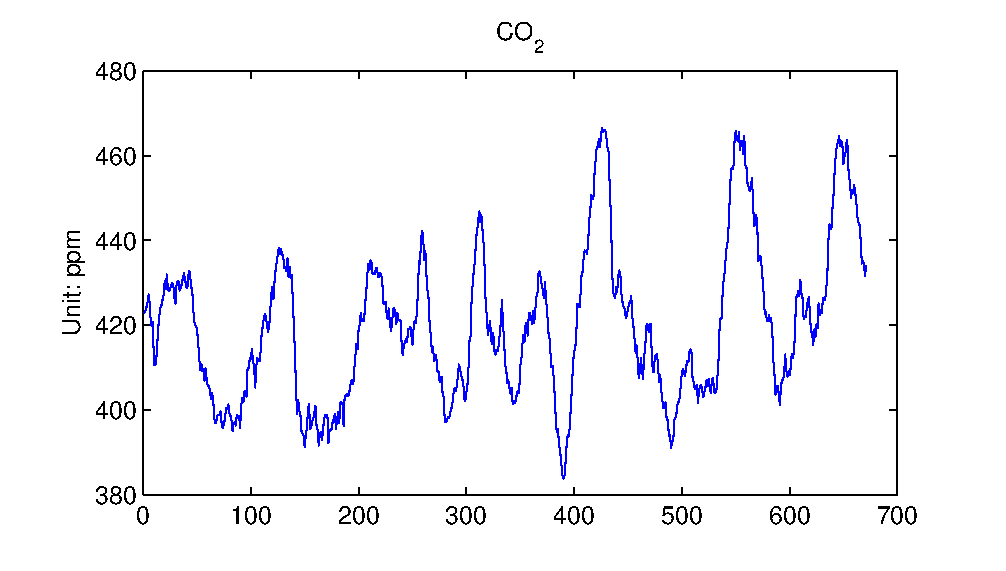
\includegraphics[width=\textwidth]{./fig/co2.eps}
                \caption{$CO_{2}$}
  \end{subfigure}
  \begin{subfigure}{0.32\textwidth}
                \centering
    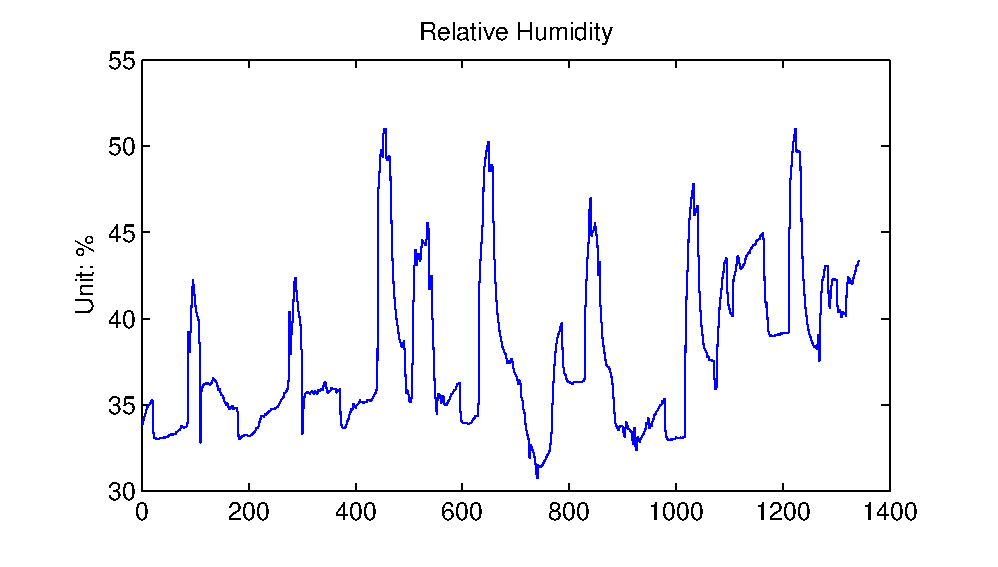
\includegraphics[width=\textwidth]{./fig/rh.eps}
                \caption{Humidity}
  \end{subfigure}
  \begin{subfigure}{0.32\textwidth}
                \centering
    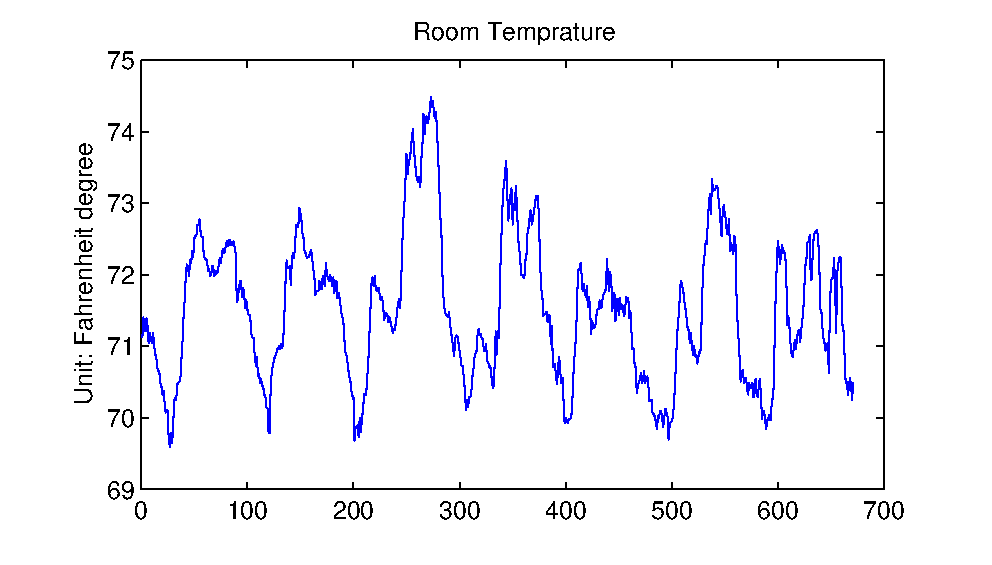
\includegraphics[width=\textwidth]{./fig/rmt.eps}
                \caption{Room Temperature}
  \end{subfigure}
  %row2
  \begin{subfigure}{0.32\textwidth}
                \centering
    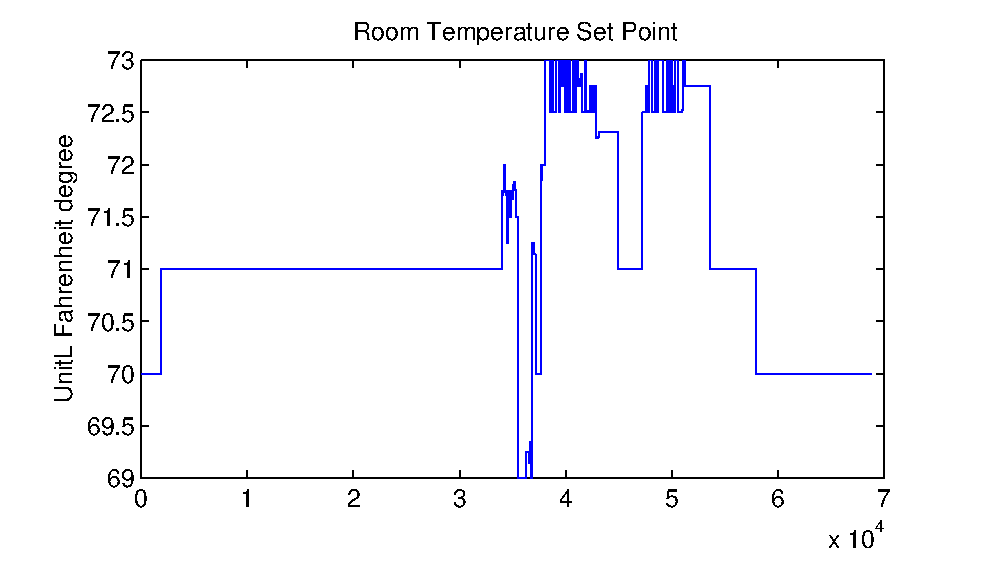
\includegraphics[width=\textwidth]{./fig/stpt.eps}
                \caption{Room Temperature Set Point}
  \end{subfigure}
  \begin{subfigure}{0.32\textwidth}
                \centering
    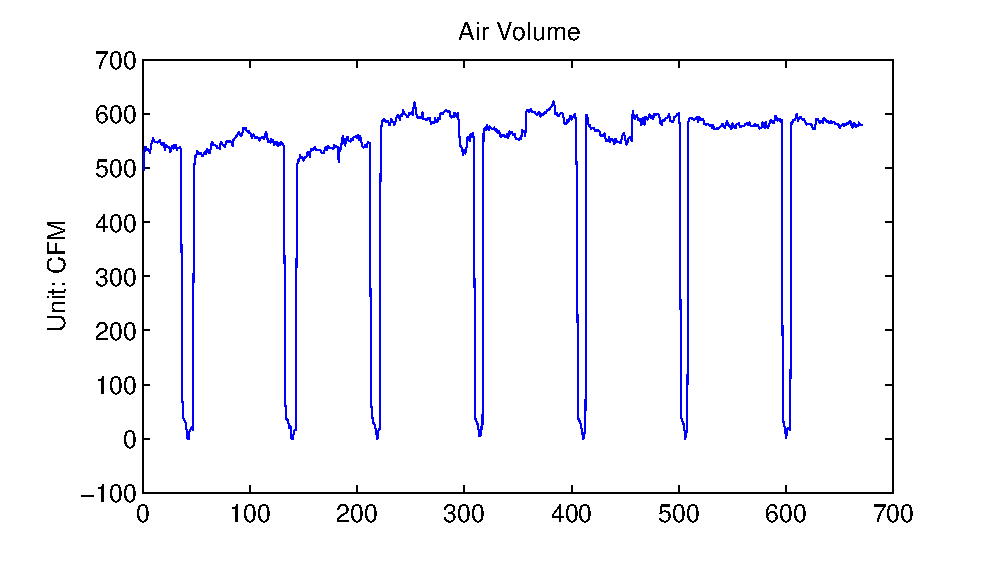
\includegraphics[width=\textwidth]{./fig/vav.eps}
                \caption{VAV Air Volume}
  \end{subfigure}
  \begin{subfigure}{0.32\textwidth}
                \centering
    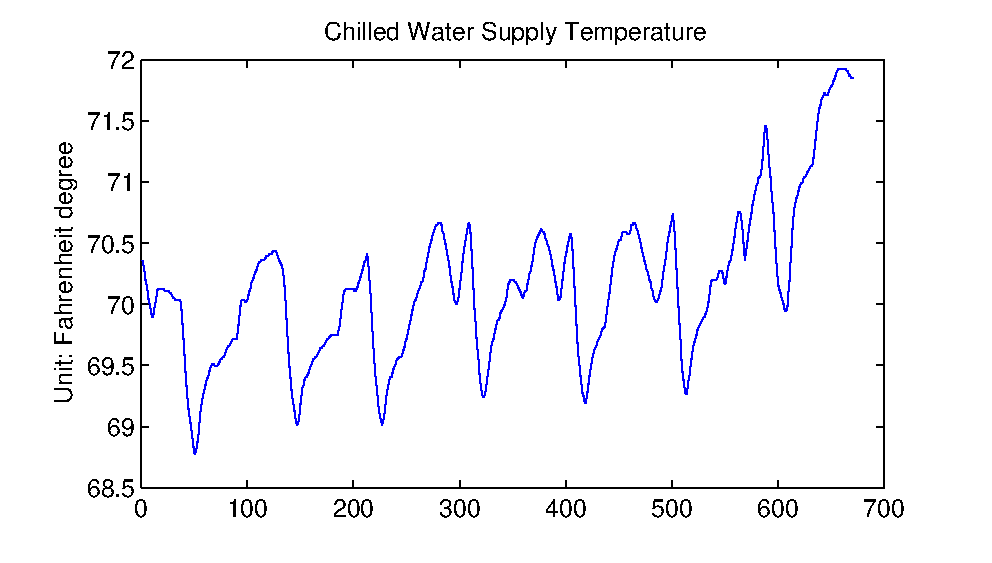
\includegraphics[width=\textwidth]{./fig/cwt.eps}
                \caption{Chilled Water Supply Temperature}
  \end{subfigure}
\caption{Different types of sensors occupy different amplitude bins in the time domain with different short term dynamics.}
\label{fig:example}
\end{figure*}

\subsubsection{Data Features}
A signal\footnote{In this paper, we use the term ``signal'', ``trace'' and ``time series'' \textit{interchangeably}.} in the time domain is a trend of sensor reading. 
Different types of sensor generally have different amplitudes that can be separated and binned,  
%occupy distinct amplitude bins, 
as demonstrated in Figure~\ref{fig:example}. 
Similar to piecewise aggregated approximation (PAA~\cite{paa}) -- where the mean is calculated in a fixed-length window -- 
we compress the signal by computing a set of summary statistics over fixed-length windows. 
%we compress a signal in a time window with summary statistics that characterize the behavior of the signal in that window.
%characterize a windowed signal in the time domain with 
%standard statistical features which are summarized in .
Table~\ref{table:fd} shows a summary of the statistics we calculate. %we use to vectorize a time window.


\begin{table}[h]
\centering
\begin{tabular}{r|l|l}
\hline
Category                   & Statistical Function & \multicolumn{1}{l}{Acronym} \\ \hline\hline
\multirow{2}{*}{Extreme}   & Minimum                 & min                          \\ \cline{3-3} 
                           & Maximum                 & max                          \\ \hline
\multirow{2}{*}{Average}   & Median                  & emd                          \\ \cline{3-3} 
                           & Root Mean Square        & rms                          \\ \hline
\multirow{2}{*}{Quartiles} & 1st and 3rd Quartiles   & 1q, 3q                       \\ \cline{3-3} 
                           & Inter-quartile range    & iqr                          \\ \hline
\multirow{3}{*}{Moments}   & Variance                & var                          \\ \cline{3-3} 
                           & Skewness                & skew                         \\ \cline{3-3} 
                           & Kurtosis                & kurt                         \\ \hline
Shape                      & Linear Regression Slope & slope                        \\ \hline
\end{tabular}
\caption{Statistical features extracted in window level for each time series data.}
\label{table:fd}
\end{table}

Our feature extraction process consists of three steps.
First, each sensor trace is segmented into N non-overlapping hour-long windows. Second, within each time window, we compute the statistics shown above. 
%This produces a vector where each component is a a %statistic over the window. %slides over the entire trace, such as 
For example, the $MIN$ vector is computed as follows: 
$MIN = \{min^{1}, min^{2}, ..., min^{N}\}$, where N is the number of time windows. We compute a similar vector for each statistic show in the table.
%Each vector, reflects short term changes that are useful for classification. 
Third, we compute a statistical summary of these vectors. For each vector we compute the minimum, maximum, median and variance, resulting in a feature 
vector containing 44 variables:
\begin{displaymath}
\begin{split}
F = \{min(MIN), max(MIN), \\ 
median(MIN), var(MIN),\\
...\\
min(SLOPE), max(SLOPE), \\
median(SLOPE), var(SLOPE)\}
\end{split}
\end{displaymath}
$F$ is the data feature vector for each sensor trace used in our study.


%First, 
%we segment each timeseries into hour-long windows and calculate the given statistics. %the above features within each window. 
%Then, we
%Since computing over features these short time windows will produce too much information as well as noise; 
%therefore we compute the statistics of the accumulated features from windowed slices as the final feature set. 

\subsubsection{Name Features}
Sensor point names are short text strings with several concatenated abbreviations, as shown in Table~\ref{table:ex}. 
To vectorize a point name, we convert all alpha characters to lower case and trim out numerical characters. 
For example, \texttt{Zone Temp 2 RMI204} becomes \texttt{\{zone, temp, rmi\}}. 
%To capture possible variants of abbreviations in point names, e.g., ``tmp'' and ``temp'' for temperature, we adopt $k$-mers \cite{leslie2004mismatch} as our features. 
We use $k$-mers \cite{leslie2004mismatch} to capture variations in type abbreviations, e.g., ``tmp'' and ``temp'' for temperature.
The term $k$-mer refers to all the possible substrings of length $k$, which are contained in a string. This feature is often used in protein and gene sequence analysis and 
it helps measure sequence similarity without requiring alignment. 

We limit the k-mers computation within a word boundary.
In general, having too small a value for $k$ will increase the chance for all the k-mers to overlap, making points less differentiable.
Therefore, we compute all k-mers of length 3 and 4 for each point name.
For example, \texttt{\{zone, temp, rmi\}} yields a set of k-mers \texttt{\{zon, one, tem, emp, rmi\}} when $k$=3.
A dictionary of k-mers is constructed with all the k-mers generated from each point name. 
Each point name is converted into a feature vector based on the frequency of k-mers in it. 
For example, a set of k-mers \texttt{\{zon, tem, emp, zon\}} will be transformed to a vector
\texttt{(2,0,1,1,0)} with the dictionary \texttt{\{zon, one, tem, emp, rmi\}}, meaning \texttt{zon} occurs twice, \texttt{one} does 
not appear, and so forth. 
This feature representation of point names will be used for examining classification performance.


\subsection{Knowledge Transfer}
The use of transfer learning is motivated by the fact that people often have one or only a few buildings labeled of which they want to take advantage to aid the labeling of a new buidling.
In our sensor type classification setting, we assume that we are provided with some labeled examples only from the training domain but do not have any labeled ones from the testing domain. 
Transfer learning fits such a scenario well in that it exploits knowledge gained from one domain\footnote{A ``domain'' particularly refers to a data set  in this paper.} where labeled data is abundant to help classify examples in a new related domain. 
Such knowledge transfer is possible when the training domain and the test domain have the same set of class labels. 
The reason that traditional supervised learning techniques is not successful in transferring knowledge across domains in our case is because it usually requires training and the testing examples sampled i.i.d. from the same distribution, which is not the case for our problem.

%For example, the classiers can be trained from several relevant domains or built using different learning algorithms on the same domain.
To encapsulate the information from one labeled building and transfer across buildings, we construct a few classifiers with different learning algorithms on the same set of data features from an existing building. 
Each different classifier usually contains a different perspective of the knowledge on the building, due to the inductive bias of the specific learning model. 
We refer to these different classifiers as {\it base} models\footnote{We use the term ``model'' and ``classifier'' {\it interchangeably} in this paper.} and will combine them for classification on the new building.
We will discuss about the choice of data features for classifier training in the evaluation.


\subsection{Locally Weighted Ensemble}
Different models can be effective at different regions or structures in the new testing building, and no single model can perform well on all examples. 
Ideally, we want to combine the knowledge in the base models, rather than only using any particular model, to more effectively transfer the knowledge to the new building. 
% A natural choice is model averaging that additively combines the predictions of multiple base learners. 
% However, the existing model averaging methods for traditional supervised learning usually assign global weights to models, which are either uniform (e.g., in Bagging~\cite{bagging}) or proportional to the training accuracy (e.g., in Boosting~\cite{boosting}), or simply relying on a specific model (e.g., single model classification).
% Such global weighting schemes may not perform well in transfer learning because different testing examples may favor predictions from different base models. 
% For example, when the base models carry conflicting concepts at a testing example, the optimal choice would be a model that better represents the distribution underlying the example.
We employ a locally weighted ensemble~\cite{lwe} to weight the predictions from base classifiers. 
The weight is computed per model per example based on the similarity between the model and the local structure of the target example. 
The similarity is measured by comparing neighborhood graphs which we will explain in the next section. 
Such local weighting will favor models whose predicted local structure is close to the true local structure of the target example in the new testing domain. 
Let $x$ be the data feature vector of an example in the new building and $y$ be its predicted class label. Given a set of $k$ base models $M_1, \dots, M_k$ and the new testing set $D_T$ represented in the data feature view, the general Bayesian model averaging rule to estimate the posterior distribution of $y$ is,
\begin{equation}\label{eq_lwe}
p(y|x)=\sum_{i=1}^k p(y|x,D_T,M_i) p(M_i|D_T)
\end{equation}
where $p(y|x,D_T,M_i) = p(y|x,M_i)$ because $x \in D_T$ and $p(y|x,M_i)$ is actually the prediction on $x$ by $M_i$. And $p(M_i|D_T)$ is the probability to choose $M_i$ given the testing set $D_T$. As $x \in D_T$, $p(M_i|D_T)$ equals to $p(M_i|x)$ which is the locally adjusted weight for $M_i$ and Eq.~\ref{eq_lwe} becomes,
\begin{equation}\label{eq_sum}
p(y|x)=\sum_{i=1}^k w_{x}^{M_i} p(y|x, M_i)
\end{equation}
where $w_{x}^{M_i} = p(M_i|x)$ and intuitively, a model $M_i$ should have higher weights for $x$ if $M_i$ predicts a similar local structure of $x$ to the true one.
We will next explain how the weight is calculated per example.

\subsection{Graph-based Weight Estimation}\label{sec:gwe}
% If $p(y|x)$ is known, we can estimate the weights $w_{x}^{M_i}$ for each model by minimizing the square error between its prediction and the ground truth. 
% However, in practice the truth value of $p(y|x)$ for a new building is not available a priori . 
% The main task becomes to properly define the similarity between classifier's predicted structure and the true structure. 
We quickly summarize the graph-based weight estimation in~\cite{lwe} and describe our two adjustments which are customized for our problem.
Following the assumption~\cite{cluster} that $p(y|x)$ is not expected to change much in a dense area where $p(x)$ is high, 
% which means the decision boundary probably exists in areas with smaller $p(x)$.
~\cite{lwe} performs clustering on the new testing set and assume the boundaries between clusters represent areas where $p(x)$ is small.
If the clustering boundary for the region where $x$ locates agrees with the decision boundary of $M_i$, 
% we assume that $p(y|x,M_i)$ is similar to the true $p(y|x)$ around $x$, which means 
a larger weight is assigned to $M_i$ at $x$.
In other words, if the predictions of $M_i$ on the area surrounding $x$ have higher consistency with the clustering results, $M_i$ would have a larger weight at $x$. 

Based these observations, the weight is estimated with a graph-based algorithm.
To compute the $w_{x}^{M_i}$ for $M_i$ at example $x$, we construct two neighorhood graphs: 
$G_M = (V, E_M)$ and $G_C = (V, E_C)$, for classification and clustering respectively, 
where each vertex is an example and $V = D_T$. In $G_M$, an edge exists between two vertices (denoting the two examples are ``neighbors'') if and only if $M_i$ predicts the same label for these two examples. Likewise, in $G_C$, an edge exists between two vertices if and only if these two examples reside in the same cluster.
If the neighbors of $x$ on both graphs significant overlap, then $M_i$ will be assigned a larger weight.
So the weight $w_{x}^{M_i}$ for $M_i$ at $x$ is proportional to the similarity of the two graphs:
\begin{equation}\label{eq_sim}
w_{x}^{M_i} \propto s(G_M, G_C|x) = \frac {|V_M \cap V_C|} {|V_M \cup V_C|}
\end{equation}
where $V_M$ ($V_C$) is the set of neighbors of $x$ on graph $G_M$ ($G_C$), |$\cdot$| is the cardinality of a set, and $s(G_M, G_C|x)$ is the similarity between two graphs. 
Figure~\ref{fig:graph} illustrates an example of neighborhood graphs for an example $x$ (in grey circle): model 1 has a similarity of 0.75 while model 2 has 0.5.

\begin{figure}[h]
\centering
    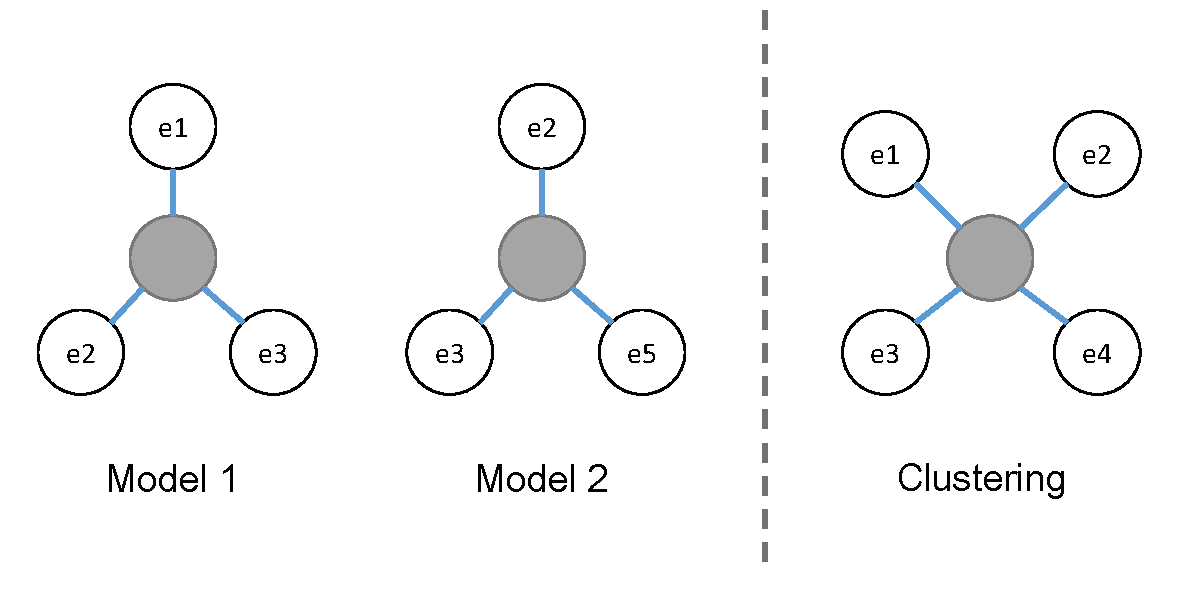
\includegraphics[width=0.4\textwidth]{./fig/lwe_graph}
\caption{An example of local neighborhood graphs of $x$ (in grey circle).}
\label{fig:graph}
\end{figure}

With Eq.~\ref{eq_sim} defined, the weight for each $M_i$ is calculated by normalizing among all similarity scores:
\begin{equation}\label{eq_norm}
w_{x}^{M_i} = \frac {s(G_{M_i}, G_C|x)} {\sum_{i=1}^k s(G_{M_i}, G_C|x)}
\end{equation}
And the final prediction for $x$ is simply $\hat y = argmax_y \enspace p(y|x)$ as $p(y|x)$ is defined in Eq.~\ref{eq_sum}.

\subsubsection{Distance-based Adjustment}
We notice in some cases the original similarity definition can be problematic. Consider the case as shown in Figure~\ref{graph_dist}, there are two neighbors on both of the graphs for the two models and the distance between vertices are marked on the edge. Since the original similarity definition only considers the number of neighbors, both models will be assigned the same weight of 0.5 in this case while obviously model 1 ought to have a higher weight because the neighbors on
the left graph are closer to the target example.
To fix the issue, we include the distance between examples into consideration, the adjusted similarity is:
\begin{equation}\label{d_sim}
s^\ast(G_M, G_C|x) = 1 - \frac {\sum d_{V_I}/|V_I|} {\sum d_{V_U}/|V_U|}
\end{equation}
where $V_I = V_M \cap V_C$, $V_U = V_M \cup V_C$, and $\sum d_{V_I}$ is the sum of distance between $x$ to its neighbors in $V_I$ (likewise for $\sum d_{V_U}$).

\begin{figure}[h]
\centering
    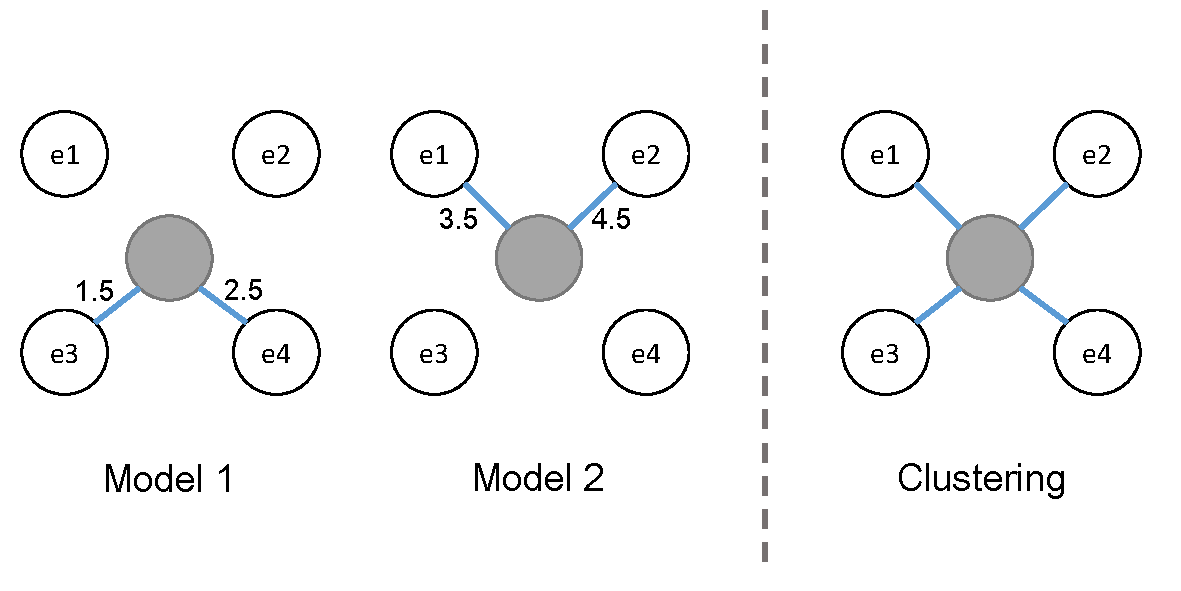
\includegraphics[width=0.4\textwidth]{./fig/lwe_d_graph}
\caption{An example of local neighborhood graphs of $x$ with distance into consideration.}
\label{graph_dist}
\end{figure}

\subsubsection{Thresholding-based Adjustment}
The use of weighted average decision for $x$ among base classifiers is reasonable when at least some of these classifiers perform well on $x$. However, the similarity $s(G_{M_i}, G_C|x)$ for $M_i$ is expected to be small when the predictions of $M_i$ around $x$ conflict with its true local structure. 
In such a case, still adopting the decision from the classifier might not be a reasonable choice. 
Since $s(G_{M_i}, G_C|x)$ reflects the consistency between classifier predictions and cluster structure, we use the average similarity score over all $M_i$ on $x$ as a discriminator to limit the usage of these base classifiers.
As an adjustment before the normalization of similarity scores, we check the average similarity score with,
\begin{equation}\label{ave_sim}
 \bar s_x = \frac {1}{k}\sum_{i=1}^k s(G_{M_i}, G_C|x)
\end{equation}
We will continue with the ensemble prediction only if $\bar s_x$ is larger than a threshold $\delta$, and we will discuss the choice of $\delta$ in the evaluation section.


\subsection{Clustering with Non-parametric Bayesian}
\label{sec_clustering}
In our transfer learning based approach, data density $p(x)$ is exploited via its latent clustering structure. We choose Gaussian Mixture Model (GMM) \cite{zivkovic2004improved}, a partitional clustering algorithm, to perform the clustering.

In GMM, the cluster label for every instance is treated as a latent variable, which is drawn from a multinomial distribution $p(c)$, i.e., $p(c)\propto\alpha_c$, where $\forall c, \alpha_c\ge0$ and $\sum_c\alpha_c=1$. In any given cluster $c$, the conditional data likelihood of an instance $x$ is specified by a multivariate Gaussian distribution. To reduce the number of parameters to estimate, we choose the isotropic Gaussian in our solution,
\begin{equation}
p(x|c)=(2\pi\sigma^2)^{-d/2}\exp{-\frac{(x-\mu_c)^\mt (x-\mu_c)}{2\sigma^2}}
\end{equation}
where the variance $\sigma^2$ is shared by all the clusters. $\{\alpha_c, \mu_c\}^k_{c=1}$ and $\sigma$ are considered as model parameters in GMM.

However, in GMM, we need to manually specify the number of clusters for a given input data set; and the clustering result of GMM is very sensitive to such setting. More importantly, in our study, usually there is more than one pattern in the point names even for the same type of sensors; therefore we cannot assume one class has only one cluster. It is impossible for us to predefine those optimal cluster sizes. To make clustering feasible on the new building, we appeal to a non-parameter Bayesian solution: we assume the model parameters $(\alpha, \mu)$ in each cluster are also random variables, which are drawn from a Dirichlet Process prior \cite{dp}.

A Dirichlet Process $DP(G_0, \eta)$ with a base distribution $G_0$ and a scaling parameter $\eta$ is a distribution over distributions~\cite{dp}. The base distribution $G_0$ specifies the prior distribution of model parameters, e.g., mean parameter $\mu$ in each cluster, and the scaling parameter $\eta$ specifies the concentration of samples drawn from the DP, e.g., cluster proportion $p(c)$. An important property of the DP is that though the draws from a DP have countably infinite size, they are discrete with probability one, which leads to a probability distribution on partitions of the data. The number of unique draws, i.e., the number of clusters, varies with respect to the data and therefore is random, instead of being pre-specified.

As a result, with the introduced $DP(G_{0}, \eta)$ prior, data density in a given collection of instances can be expressed using a stick-breaking representation
\cite{sethuraman1994constructive}:
\begin{equation}\label{eq_dp_density}
p(x)=\sum_{c=1}^\infty \alpha_c \mathcal{N}(x|\mu_c,\sigma)p(\mu_c|G_0)
\end{equation}
where $\alpha={\alpha}_{c=1}^\infty\sim Stick(\eta)$ represents the proportion of clusters in the whole collection. The stick-breaking process $Stick(\eta)$ for the cluster proportion parameter $\alpha$ is defined as: $\alpha'_c\sim Beta(1, \eta), \alpha_c=\alpha'_c\prod_{i=1}^{c-1}(1-\alpha'_i)$. Since the variance $\sigma^2$ is fixed in all clusters, we use a conjugate prior for $\mu$ in $G_0$, i.e., for $\forall c, \mu_{ci}\sim \mathcal{N}(a,b)$, with the assumption that each dimension in $\mu_c$ is independently drawn from a univariate Gaussian. This will greatly simplify the later on inference procedure.

Because the data density distribution defined in Eq~\eqref{eq_dp_density} only has finite support at the points of $\{\alpha_c, \mu_c\}^k_{c=1}$, we can calculate the posterior distribution of latent cluster labels in each unlabeled instance to discover the clustering structure. Following the sampling scheme proposed in \cite{neal2000markov}, we appeal to a Gibbs sampling method to infer the posterior of cluster membership. Detailed specifications of this sampling algorithm can be found in \cite{neal2000markov}.


{\bf Putting it all together:} Algorithm~\ref{algo} summarizes our transfer learning algorithm for the sensor type classification across buildings. We start from training a few base classifiers with the data features and labels of examples in a source building. We also generate clusters with DP on the name features of examples in the target building. For each example $x$ in the target building, we measure the local similarity score for each base classifier. If the average similarity is significant enough, we compute the weight for each classifier at $x$ by normalizing the similarity score. Finally we calculate the weighted sum of predictions from all base classifier and obtain the label $y$ for $x$.

\begin{algorithm}[ht]
 \caption{Transfer Learning for Sensor Type Classification}
 \label{algo}
 %\SetAlgoLined
 {\bf Input}: Data features of the source building $\mathcal{D_S}=\{x^D_1,x^D_2,\dots,x^D_n\}$ and their labels $\mathcal{Y_S}=\{y_1,y_2,\dots,y_n\}$  data features of the target building $\mathcal{D_T}=\{x^D_1,x^D_2,\dots,x^D_m\}$, and name features of the target building $\mathcal{P_T}=\{x^P_1,x^P_2,\dots,x^P_m\}$\\
 {\bf Output}: predicted labels of the examples in target building $\mathcal{Y}$\\
 Initialize: Generate clusters with $DP(G_{0}, \eta)$ on $\mathcal{P_T}$\\
 Train $k$ classifiers $M_1, \dots, M_k$ based on $\mathcal{D_S}$ and $\mathcal{Y_S}$\;

\For{$x^D$ in $\mathcal{D_T}$}{
Construct neighborhood graphs $G_M$ and $G_C$ for $x^D$ as defined in Section~\ref{sec:gwe} for each $M_i$;\\
Compute the similarity score for each $M_i$ with Eq.~\ref{d_sim};\\
Check the average similarity score $\hat s_x$ over all $M_i$ with Eq.~\ref{ave_sim};\\
If $\hat s_x > \delta$, then use Eq.~\ref{eq_norm} and Eq.~\ref{eq_sum} to predict the label $y$;
}
\end{algorithm}
